\documentclass[a4paper,12pt]{article}

\usepackage{amsmath,amssymb,amsthm,tikz}
\usetikzlibrary{calc,arrows.meta}
\usepackage[margin=20mm]{geometry}
\usepackage{hyperref}

\setlength{\parindent}{0pt}
\setlength{\columnsep}{1cm}

\begin{document}

%\twocolumn

\thispagestyle{empty}

\begin{center}
{\Large Sample Assignment 7}\\
{\Large Discussed on 2020-11-05,}\\
{\em Not graded} 
\end{center}

\noindent


\vspace{10pt}
{\bf Question 1 (Polynomial HashCodes for Strings).}\\
You have $4$ different ASCII strings: $\textcolor{blue}{\mathtt{ABCD}}$, 
$\textcolor{blue}{\mathtt{ABD}}$, 
$\textcolor{blue}{\mathtt{ACD}}$, 
$\textcolor{blue}{\mathtt{BCD}}$, and you want to compute 
Java/Scala-style hash function and insert them (in this order) into a
hash table $H$ with $5$ slots: $H[0],\ldots,H[4]$. 

{\bf (A)} Compute the (uncompressed) hashcode values for all the $4$ string values. 
Your hashcode function $h_1(s) = p(31)$ (value of a polinomial for argument $z = 31$), where
$p(z)$ is defined as follows:
$$p(z) = \sum\limits_{i=0}^{L-1} \operatorname{ord}(c[i]) z^{L-1-i}.$$
Here $L$ is the length of the string $s$.
By $c[i]$ we denote the $i$th character of the input string $s$
($i = 0,1,\ldots,L-1$). 
Polynomial is computed in a $4$-byte integer register; if the 
integer register overflows, we only use the last four bytes.  
In this exercise all the strings are sufficiently short and the overflow does not happen. 

{\em Note.} By $\operatorname{ord}(c)$ in this polynomial we denote
the ASCII code of some character {\tt c}; these codes are integers in $[0;255]$. 
(See the ASCII codes: \url{http://www.asciitable.com/}.) 

\vspace{10pt}
{\bf (B)} Write the arithmetic expression to evaluate $h_1(\textcolor{blue}{\mathtt{ABCD}})$ with the {\em Horner's method}
using only three multiplications and three additions (and no intermediate variables can be stored). 

\vspace{10pt}
{\bf (C)} Compute the compressed hash values for the same 4 strings
($\textcolor{blue}{\mathtt{ABCD}}$, 
$\textcolor{blue}{\mathtt{ABD}}$, 
$\textcolor{blue}{\mathtt{ACD}}$, 
$\textcolor{blue}{\mathtt{BCD}}$) modulo $5$. Namely, 
the compressed hash value is 
$$h_2(h_1(s)) = h_1(s)\;\text{mod}\;5.$$

\vspace{10pt}
{\bf (D)} Draw the four string objects in a hashtable $H$ with $5$ cells
($H[0],\ldots,H[4]$). 

\vspace{30pt}
{\em Note.} 
Here is the pseudocode of the abovementioned string hashing function $h_1(s)$ (in Python): 
\begin{verbatim}
def h1(s):
    h = 0
    for c in s:
        h = (31 * h + ord(c)) & 0xFFFFFFFF
    return ((h + 0x80000000) & 0xFFFFFFFF) - 0x80000000
\end{verbatim}

All the manipulation with masks {\tt 0xFFFFFFFF} etc. is meant to guarantee that $h_1(s)$ 
is always 4 bytes long signed integer (in Python integers are generally longer). 
Your polynomial computations will not be affected by these masks (for short strings the
value $h_1(s)$ is a positive number that does not cause 4-byte register overflow). 



% https://stackoverflow.com/questions/17016175/c-unordered-map-using-a-custom-class-type-as-the-key






\newpage

{\bf Question 1}\\
{\bf (A)} Compute the values by hand or use Python pseudocode:

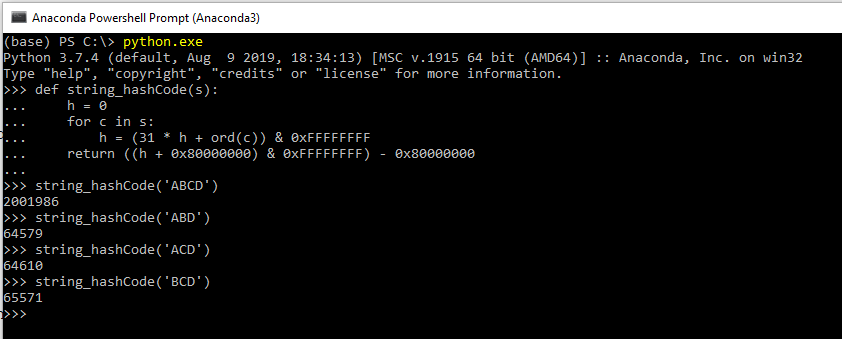
\includegraphics[width=6in]{assignment07-hashtables/python-console.png}

\vspace{10pt}
{\bf (B)} You can use Horner's method like this: 
$$h_1(\textcolor{blue}{\mathtt{ABCD}}) = ((65 \cdot 31 + 66) \cdot 31 + 67) \cdot 31 + 68.$$ 
Notice that the characters {\tt 'A'}, {\tt 'B'}, {\tt 'C'}, {\tt 'D'} have ASCII codes
$65,66,67,68$ respectively. In hexadecimal notation, the byte {\tt 'A'} is {\tt 0x41}, which 
equals $4 \cdot 16 + 1 = 65$. See \url{http://www.asciitable.com/} for details. 

{\em Note.} If Horner's method is not used, then a 3rd degree polynomial would take $3$ additions
and $6$ multiplications. This is even more inefficient for longer strings, so we should always
use the Horner's method (also used in the Python pseudocode on the previous page). 
Here is the same polynomial without Horner's method:
$$h_1(\textcolor{blue}{\mathtt{ABCD}}) = 65 \cdot 31 \cdot 31 \cdot 31 + 66 \cdot 31 \cdot 31 + 67 \cdot 31 + 68.$$ 

\vspace{10pt}
{\bf (C)} The compressed hash values are the remainders of numbers $2001986$, 
$64579$, $64610$ and $65571$ when divided by $5$ (i.e.\ they are numbers $1$, $4$, $0$, $1$ respectively). 

\vspace{10pt}
{\bf (D)} Here is the image with the hashtable (with all the 5 slots/buckets displayed). There
is one collision: two different values map to the same (compressed) value $1$. 
Hashtable is represented as an array of linked lists. 
The key $\textcolor{blue}{\mathtt{ABCD}}$ is inserted first, only then the collision with 
another key $\textcolor{blue}{\mathtt{BCD}}$ happens (so it becomes the next member in the linked list
for the bucket $H[1]$). 


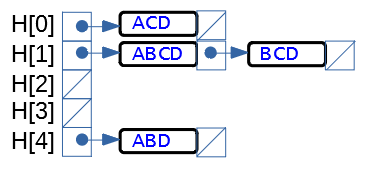
\includegraphics[width=2.5in]{assignment07-hashtables/5slot-hashtable.png}

\vspace{30pt}
{\em Note.} The hashfunction $h_1(s)$ is one of the simplest hash functions that is widely used.\\
See \url{https://docs.oracle.com/javase/7/docs/api/java/lang/String.html#hashCode()}. 



\end{document}



